\documentclass[10pt,twocolumn,letterpaper]{article}

\usepackage{cvpr}
\usepackage{times}
\usepackage{epsfig}
\usepackage{graphicx}
\usepackage{amsmath}
\usepackage{amssymb}
\usepackage{gensymb}

\usepackage{stfloats}
\usepackage{tablefootnote}

%%%%%%%% OTHER PACKAGES
\usepackage{float}
\usepackage{caption} % solve for table caption spacing 
\captionsetup[table]{skip=10pt} % to force bib position
\usepackage[section]{placeins}
\usepackage{subcaption}
\usepackage{multirow} % for tabular multi-row
\usepackage{enumitem}
\newcommand{\denselist}{\itemsep -2pt\parsep=1pt\partopsep 0pt}
\newcommand{\bitem}{\begin{itemize}\denselist}
\newcommand{\eitem}{\end{itemize}}
\newcommand{\benum}{\begin{enumerate}\denselist}
\newcommand{\eenum}{\end{enumerate}}
%%%%%%%%%%%%%%%

\usepackage[breaklinks=true,bookmarks=false]{hyperref}

\cvprfinalcopy % *** Uncomment this line for the final submission

\def\cvprPaperID{****} % *** Enter the CVPR Paper ID here
\def\httilde{\mbox{\tt\raisebox{-.5ex}{\symbol{126}}}}

% Pages are numbered in submission mode, and unnumbered in camera-ready
%\ifcvprfinal\pagestyle{empty}\fi
\setcounter{page}{1}
\begin{document}

%%%%%%%%% TITLE
\title{DPN Learner:Unsupervised Learning of Depth, Ego-Motion and Surface Normal from Video}

\author{Aman Raj\\
A53247556\\
{\tt\small amraj@eng.ucsd.edu}
% For a paper whose authors are all at the same institution,
% omit the following lines up until the closing ``}''.
% Additional authors and addresses can be added with ``\and'',
% just like the second author.
% To save space, use either the email address or home page, not both
\and
Menghe Zhang\\
A53208258\\
{\tt\small mez071@eng.ucsd.edu}
\and
Sarah Wang\\
A53276846\\
{\tt\small sawang@eng.ucsd.edu}
\and
Tingwei Yu\\
A53281022\\
{\tt\small t3yu@eng.ucsd.edu}}

\maketitle
%\thispagestyle{empty}

%%%%%%%%% ABSTRACT
\begin{abstract}

Learning to reconstruct depths and camera pose from a single image in unsupervised approach via deep convolutional network is attracting significant attention since Zhou proposed the unsupervised learning framework for the task of monocular depth and camera motion estimation from unstructured video sequences\cite{zhou2017unsupervised}. Our work extends their work by estimating depth map, camera pose and surface normal map together in an end-to-end framework. We verify that deep network approaches benefit from explicit geometric cues and constraints. Therefore, we take advantage both instance-level and semantic-level segmentation to make the framework edge-aware while using the consistency between depth and normal, yielding more robust prediction for both depths, surface normals and ego-motions. Evaluations are conducted on both outdoor(KITTI) and indoor(NYUv2) datasets. Ablation studies regarding different geometric constraints are conducted to compare their effectiveness.  

\end{abstract}

%------------------------------------------------------------------------

\section{Introduction}
Inferring camera poses, depths and surface normal of a scene at a detailed level is crucial for 3D scene understanding. Recovering these information from monocular images can be widely applied in various real-world applications. For instance, in robot navigation, this enables the robot to avoid obstacles and travel through unseen areas. The ability to estimate depth and surface normal also facilitates 3D reconstruction of the environment and can be applied in the field of augmented reality. \\
Recently, there has been large progress in unsupervised pose and depth estimation using monocular cameras. Works such as \cite{zhou2017unsupervised} has significantly reduced the human effort to obtain large quantities of ground truth color-depth image pairs for training while also yielding comparable results to supervised approaches. The key concept is to use view synthesis as supervision by warping a image in a sequence to its consecutive frames. Following works attempt to exploit more geometric cues and constraints to improve the depth results.\cite{yang2018lego} refines the estimated depth by leveraging the constraint between surface normal and depth map as well as using image gradients to represent edges where depth discontinuities can occur.  \cite{casser2018depth} takes additional instance-level segmentation information as input and predicts poses for the background and each object separately. \\
In our work, we study the effects of posing various geometric constraints on the quality of depth estimation. First, we show that by utilizing additional semantic segmentation information, the model is able to learn the boundaries of the scene objects and generate sharper depth results. Second, we investigate how edge detection lead to better depth predictions. Last, we compare the results of the normal-depth constraint used in \cite{yang2018lego} and the patch-based photometric consistency constraint used in  \cite{furukawa2010accurate}. Evaluation on the KITTI dataset demonstrates the effectiveness of different approaches.


%------------------------------------------------------------------------
\section{Related work}
\textbf{Warping-based view synthesis}
View synthesis aims to create novel view of a specific subject from images taken from other point of views. Classic paradigm for view synthesis explicitly reconstruct the accurate 3D model of the scene, then composite novel view from the input images \cite{malik1996modeling}\cite{fitzgibbon2005image}\cite{DBLP:journals/tog/ZitnickKUWS04}. Another common approach is to synthesize images without explicitly estimating the 3D geometry of the scene. For instance, Mahajan\cite{shechtman2010regenerative} proposed to move the gradients in the input images along a specific path to reconstruct the image at a novel view. Shechtman\cite{shechtman2010regenerative} proposed a patch-based optimization framework to reconstruct novel views. The end-to-end learning based framework DeepStereo\cite{DBLP:journals/corr/FlynnNPS15}, on the other hand, uses two towers to predict depth and color and fused them together to construct the novel view.  However, unlike the warping-based methods, such frameworks only work on the inputs and output, without learning intermediate predictions of geometry and correspondence. 
\\
\textbf{Unsupervised learning from videos} Unsupervised learning of visual representations has a
rich history starting from original auto-encoders work of Olhausen and Field\cite{olshausen1997sparse}. To get the visual representation from video, the general goal is to design pretext tasks for learning generic visual features, that are sparse and reconstructive, from video data that can later be re-purposed for other vision tasks. Researchers have started focusing on learning feature representations using videos. Early work such as\cite{zou2012deep} focused on inclusion of constraints via video to autoencoder framework. The most common constraint is enforcing learned representations to be temporally smooth. Similar to this, Goroshin et al.\cite{goroshin2015unsupervised} proposed to learn autoencoders based on the slowness prior. Other approaches such as Taylor et al.\cite{taylor2010convolutional} trained convolutional gated RBMs to learn latent representations from pairs of successive images. This was extended in a recent work by Srivastava et al.\cite{srivastava2015unsupervised} where they proposed to learn a LSTM model in an unsupervised manner to predict future frames.
\\
\textbf{Image segmentation}
Semantic segmentation with the goal to assign semantic labels to every pixel in an image is one of the fundamental topics in computer vision. Deep convolutional neural networks based on the Fully Convolutional Neural Network show striking improvement over systems relying on hand-crafted features on benchmark tasks. DeepLab is a state-of-art deep learning model for semantic image segmentation. The most state-of-the-art work, DeepLabv3+\cite{deeplabv3plus2018} extends DeepLabv3\cite{chen2017rethinking} to include a simple yet effective decoder module and a spatial pyramid pooling module to refine the segmentation results especially along object boundaries. Furthermore, in this encoder-decoder structure one can arbitrarily control the resolution of extracted encoder features by atrous convolution to trade-off precision and runtime.
%%%%%%%%%%%%%%%%5instance level here


%------------------------------------------------------------------------
\section{Method}
The approaches we stress here are used for jointly estimating depths, surface normal and ego-motions. The core underlying idea is inverse warping from target view to source view with awareness of 3D geometry and depth-normal consistency. 
\subsection{Network architecture}
\textbf{Depth and Normal Net}
For depth and surface normal estimation, we adopted the DispNet \cite{mayer2016dispnet} architecture which uses an encoder followed by a decoder with skip connections and multi-scale side outputs. The depth and normal net share the same encoder while having different decoders to predict depth and normals separately. Other than the final output layer which has a sigmoid function applied to enforce the predictions in an reasonable range, the other conv layers of both nets are followed by ReLU activations.\\  
\textbf{Pose Net}
We adopted the pose net architecture purposed in \cite{zhou2017unsupervised}, the input of the network is the target-source frame pair, and the output is the 6D camera pose from each target frame to the source frame. All conv layers are followed by ReLU activations except for the final output layer, where no non-linear activation is applied.
\subsection{View synthesis as supervision}
Following the notation used in \cite{zhou2017unsupervised}, given a pair of images consisting of a target frame $I_t$ and a source frame $I_s$, we can estimate the depth map $\hat{D_t}$ of the target view and the 6-DOF transformation $\hat{T}_{t\xrightarrow{}s}$ from $I_t$ to $I_s$. Thus, for any pixel $p_t$ in the target frame $I_t$, its corresponding pixel coordinate in the source frame $p_s$ can be found through perspective projection. 

\begin{equation}
    p_s \sim K\hat{T}_{t\xrightarrow{}s}\hat{D_t}(p_t)K^{-1}p_t
\end{equation}
Using this correspondence, a synthesized target view $\hat{I_s}$ can be generated from $I_s$ through bilinear interpolation. Viewing the target frame as our reference, the photometric loss can be formulated as 
\begin{equation}
    L_{vs} = \sum_s\sum_p |I_t(p) - \hat{I_s}(p)|
\end{equation}
by summing over all pixels $p$ and source images $s$. $\hat{I_s}$ is the source view $I_s$ warped to the target coordinate frame.\\
\textbf{Regularization of depth} In order to produce smooth depth results, a smooth loss is added for regularization. This loss encourages the estimated depth to be locally similar when no significant image gradient exists, that is 
\begin{equation}
    L_s = \sum_{pt}\sum_{d\in x, y}||\bigtriangledown_d^2D_t(p_t)||e^{-\alpha|\bigtriangledown_dI(p_t)|}
\end{equation}.

\textbf{Photometric pixel loss} In addition to the reconstruction loss and smooth loss, Structural Similarity(SSIM)\cite{wang2004image} loss is applied to be part of pixel loss, where
\begin{equation}
    L_{pixel} = \alpha_{pixel} \frac{(2\mu_x\mu_y + C_1)(2\sigma_{xy} + C_2)}{(\mu_x^2 + \mu_y^2 + C1)(\sigma_x^2 + \sigma_y^2 + C_2)}
\end{equation}
\subsection{Edge-aware depth estimation}
In this section, we illustrate two ways to parameterize geometric edges. First is to use the image gradient: we compute a gradient map of the target image $I_t$ and synthesized target image $\hat{I_s}$, and require the two gradient images to match as described in \cite{yang2017unsupervised}.
\begin{equation}
    L_g = \sum_{s=1}^S\sum_{x_t}M_s(x_t)||\bigtriangledown I_t(x_t) - \bigtriangledown\hat{I_s}(x_t)||_1
\end{equation}
Here, $M_s(x_t)$ is the explainablitiy mask as in \cite{zhou2017unsupervised}. Another way to parameterize edges is to jointly learn the edge map $E_t$ for the target image from semantic mask. Here we have the intervening contour cue for measuring the affinity between two pixels. Specifically, we parameterize the prediction of $E_t$ using a decoder network same to DispNet, and add another edge loss term(computed from semantic masks) to loss function.
\subsection{Depth-normal consistency constraints}
\textbf{Depth and normal orthogonality constraint} To train the normal network, we applied the depth-normal orthogonality constraint purposed in \cite{yang2017unsupervised} to our network. This could enforce the predicted surface normal to be perpendicular to its tangent plane. Where for each pixel $x_i$ in the target view, we compute sum of the absolute dot products between the estimated normal and the vectors pointing from the pixel to it's 8 neighboring pixels as shown in \ref{fig:8point}. The equation is written as,
\begin{multline}
    L_{orth} = \sum_{i\in t}\sum_{j\in Nei(i)}||[ \phi(x_j) - \phi(x_i)] \hat{N_t}(x_i)||_1 
    \\
where \phi(x) = D_t(x)K^{-1}x
\end{multline}
where $Nei(x_i)$ denotes the set of 8 neighboring pixels of $x_i$, $K$ the camera intrinsic matrix and $\hat N(x_i)$ and $\hat D(x_i)$ the estimated surface normal and depth of the corresponding pixel, respectively. We define $\phi(x_i)$ as the back-projected 3D point of pixel $x_i$ in the 3D space, thus $\phi(x_j) - \phi(x_i)$ is the vector pointing from the center pixel to the neighboring pixels in the world coordinates. \\
Since we don't have direct supervision for $N(x_i)$, training for the above equation would result into always predicting the values in $\hat{N}$ to zero. Thus we concluded an additional regularization term $L_n$ in the loss function, where we enforce the norm the predicted surface normal to be 1.
\\
\textbf{Patch-based depth and normal constraint} Through experiments we observed that by only enforcing the depth and normal orthogonality correlation could not provide our network enough geometry cues to reconstruct the surface normal.(fig. \ref{fig:KITTI_orth}) Thus, we applied the patched-based depth and normal constraint to our network based on previous works \cite{furukawa2010accurate}. For each pixel in the target image, we reconstructed a $\mu \times \mu$ patch $p$ in the 3D space with the center calculated by back-projecting the pixel (fig.\ref{fig:patch}). The orientation of the patch is given by the estimated surface normal and we assign one of its edges to be parallel to the x-axis of the target frame. Through re-projecting each patch back in to the target image $I_t$ as well as the source image $I_s$, we sample the intensities of the patch in both views through bilinear interpolation to acquire $I_{t,p_i}$ and $I_{s,p_i}$. The loss term $L_{patch}$ is then the sum of L1 difference of the intensities between each pair of patches. 
\begin{figure}
  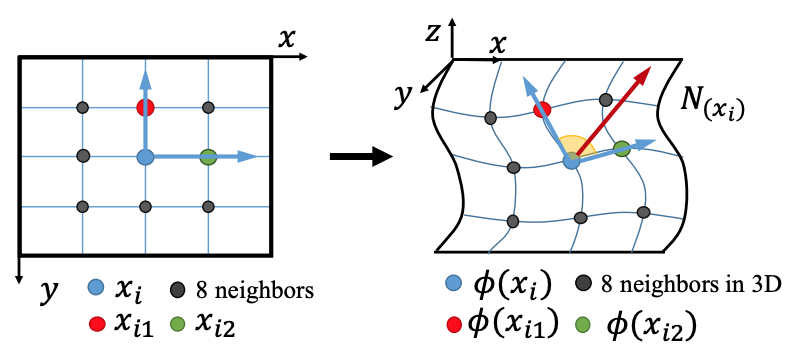
\includegraphics[width=\columnwidth ]{8point.png}
  \caption{Depth and normal orthogonality constraint. To enforce the predicted surface to be perpendicular to the tangent surface, we compute the dot product between the estimated normal and the 8 vectors pointing from the center pixel to the neighboring pixels.}
  \label{fig:8point}
\end{figure}
\begin{figure}
  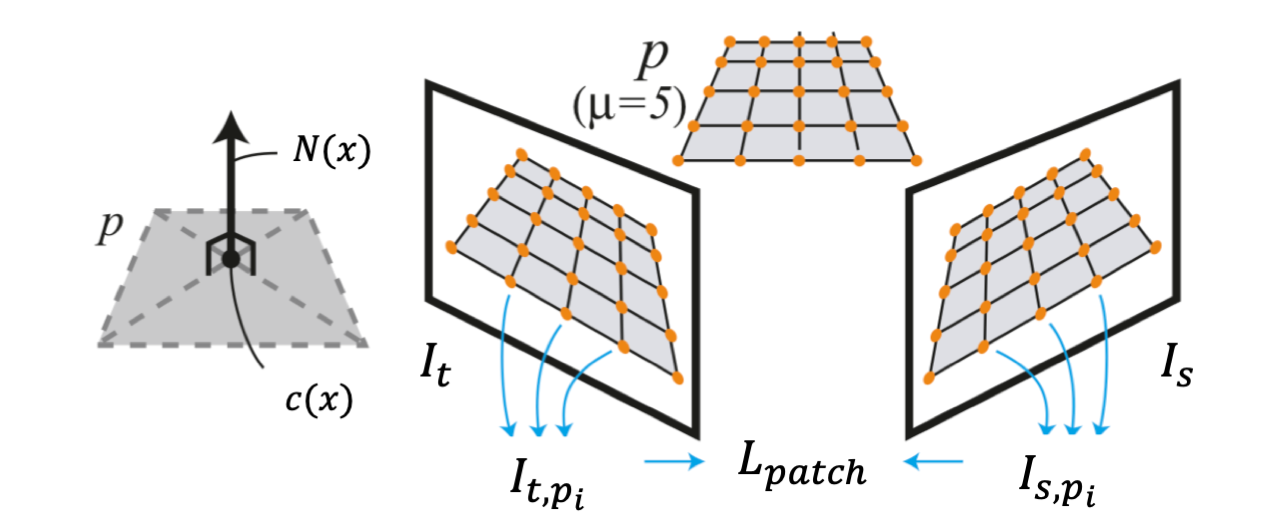
\includegraphics[width=\columnwidth ]{patch.png}
  \caption{Patched-based depth and normal constraint. For each pixel, we reconstruct a patch in the 3D space. The center of the patch $c(x)$ is obtained by back-projecting the pixel with the estimated depth, intrinsic matrix and extrinsic matrix. The orientation of the patch is given by estimated normal $N(x)$.}
  \label{fig:patch}
\end{figure}

\subsection{Object motion model with semantic priors}
Adapting the work of \cite{casser2018depth} which explicitly models the 3D motion of dynamic objects along with ego-motion of camera, we extend this work further by integrating semantic information of scene to improve depth prediction. Intuitively, semantic information encodes spatial constraints which can explain depth and normal discontinuities. Our depth network takes as input RGB sequence along with corresponding semantic segmentation(pixel-wise), encoded in one-hot encoding format. The ego-motion network $\phi_{E}$ is used to predict egomotion of static background and object motion model $\phi_{M}$ is used to predict motion of individual dynamic objects. $\phi_{E}$ and $\phi_{M}$ share the same architecture but different inputs. 

We define instance-aligned segmentation masks $(S_{1}, S_{2}, S_{3})$ for corresponding sequence $(I_{1}, I_{2}, I_{3})$. In order to compute egomotion motion of static scene only, we define static scene binary mask $(O_{1}, O_{2}, O_{3})$ where $O_{i}'s$ are binary complement of $S_{i}'s$. The static binary mask is applied to all images in sequence by element-wise multiplication to mask out dynamic objects before feeding the sequence to ego-motion model:
\begin{multline}
    V = O_{1} \odot O_{2} \odot O_{3} 
    \\
E_{1\rightarrow2}, E_{2\rightarrow3} = \phi_{E}(I_{1} \odot V, I_{2} \odot V, I_{3} \odot V) 
\end{multline}

To compute object motion model, we first apply ego-motion estimates to get warped RGB sequences $(\hat I_{1\rightarrow2}, I_{2}, \hat I_{3\rightarrow2}$ and instance-aligned segmentation sequences $(\hat S_{1\rightarrow2}, S_{2}, \hat S_{3\rightarrow2}$. Now, for every object instance in image, the object motion estimate $M^{(i)}$ of the \textit{i}-th object is computed as:

\begin{multline}
        M_{1\rightarrow2}^{(i)}, M_{2\rightarrow3}^{(i)} = \phi_{M}(\hat I_{1\rightarrow2} \odot \psi_{i}(\hat S_{1\rightarrow2}),
    \\
    I_{2} \odot \psi_{i}(S_{2}), \hat I_{3\rightarrow2} \odot \psi_{i}(\hat S_{3\rightarrow2})
\end{multline}

where $M_{1\rightarrow2}^{(i)}, M_{1\rightarrow2}^{(i)} \in \mathbb{R}^{6}$ and $\psi_{i}(S_{1})$ returns binary mask only for object \textit{i} in  $S_{1}$. Now, corresponding to these motion estimates, inverse warping is done to move the objects according to predicted motions. This is done by first warping the full image using motion estimate and then masking out the corresponding object. For example, $\hat I_{1\rightarrow2}^{(i)}$ is obtained by using motion estimate $M_{1\rightarrow2}^{(i)}$. Final warped image is a combination of warped static background and individual warping of each dynamic object. Final warped image $\hat I_{1\rightarrow2}^{(F)}$ given by:

\begin{multline}
\hat I_{1\rightarrow2}^{(F)} = \hat I_{1\rightarrow2} \odot V + \sum_{i=1}^{N} \hat I_{1\rightarrow2}^{(i)} \odot \psi_{i}(S_{2})
\end{multline}

Equivalent for $\hat I_{3\rightarrow2}^{(F)}$ can be found using above equation. We also impose object size constraint as in \cite{casser2018depth}, to make sure the network is learning reasonable depth matching object motion estimates. 
\begin{figure}
    \centering
    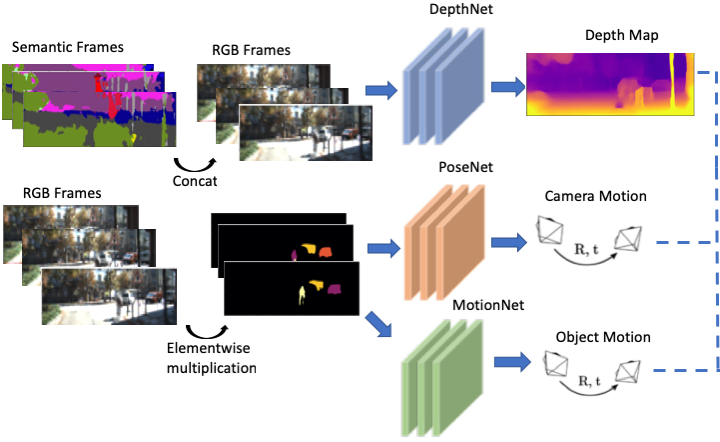
\includegraphics[width=\linewidth]{architecture.png}
    \caption{Our unsupervised architecture contains DepthNet, PoseNet and MotionNet}
    \label{fig:arch}
\end{figure}
%%%%%%%%%%%%%%% RESULT
\begin{figure}[t]
  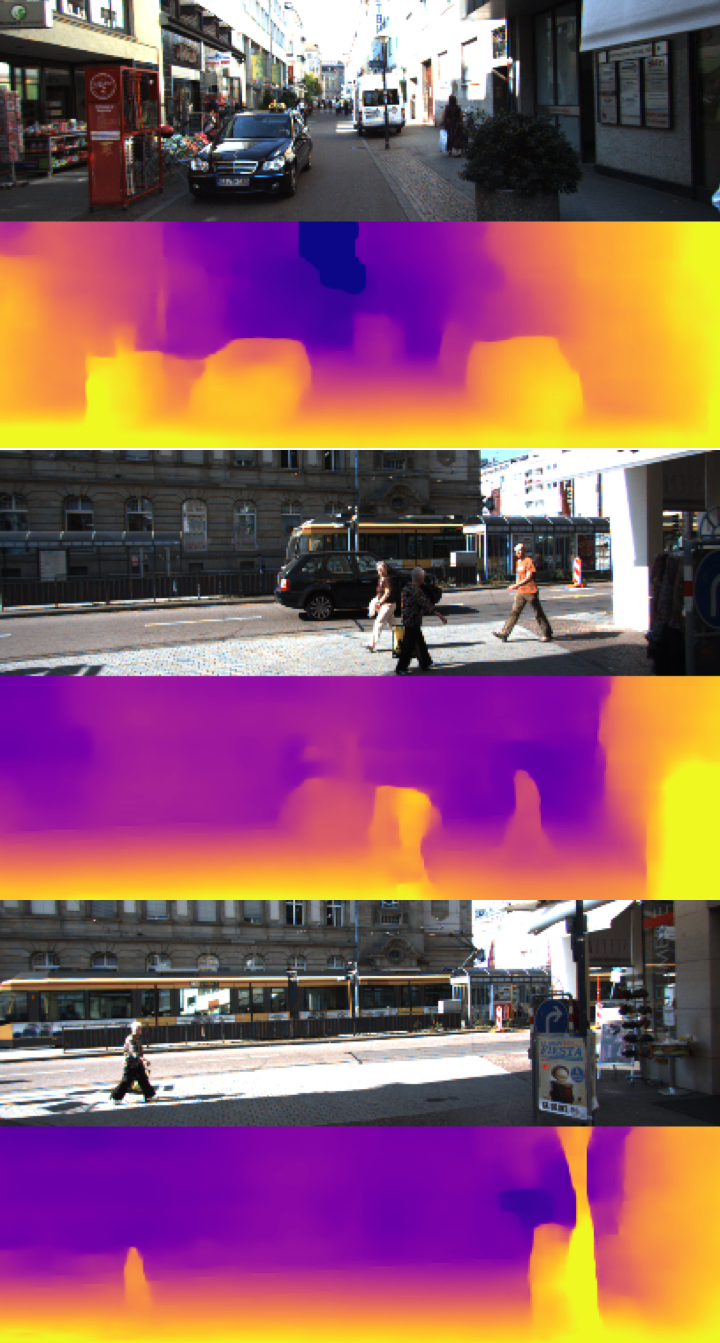
\includegraphics[width=\columnwidth]{dresult.png}
  \caption{Depth-result using our best model}
  \label{fig:depth_result}
\end{figure}
%------------------------------------------------------------------------

\begin{table*}[htbp]
\centering
\begin{tabular}{ c||c| c c c c|c c c  }
 \hline
  \multirow{2}{*}{Method} & \multirow{2}{*}{Supervised} & \multicolumn{4}{c|}{Error-related metrics} & \multicolumn{3}{c}{Accuracy-related metrics}\\
  &   & Abs Rel & Sq Rel & RSME & RSME log & $\delta < 1.25$ & $\delta < 1.25^2$ & $\delta < 1.25^3$\\
 \hline
 Eigen \textit{et al.} \cite{eigen2014depth} Coarse & Depth & 0.214 & 1.605 & 6.653 & 0.292 & 0.673 & 0.884 & 0.957 \\

  Eigen \textit{et al.} \cite{eigen2014depth} Fine & Depth & 0.203 & 1.548 & 6.307 & 0.282 & 0.702 & 0.890 & 0.957 \\

  Liu \textit{et al.}  \cite{liu2016learning} & Depth & 0.202 & 1.614 & 6.523 & 0.275 & 0.678 & 0.895 & 0.965 \\

  Godard \textit{et al.} \cite{godard2017unsupervised}  & Pose & 0.148 & 1.344 & 5.927 & 0.247 & 0.803 & 0.922 & 0.964 \\

  Zhou \textit{et al.} \cite{zhou2017unsupervised} updated & No & 0.183 & 1.595 & 6.709 & 0.270 & 0.734 & 0.902 & 0.959\\

  Yin \textit{et al.} \cite{yin2018geonet} & No & 0.155 & 1.296 & 5.857 & 0.233 & 0.793 & 0.931 & 0.973 \\

  \hline
  \textbf{Ours[]} & No & \textbf{0.133} &     \textbf{0.905} &     \textbf{5.181} &     \textbf{0.208} &     \textbf{0.825} &     \textbf{0.947} &     \textbf{0.981}\\
  
  Ours(joint training, orthogonality constraint) & No & 0.2488 & 4.9442 & 8.1843 & 0.3169 & 0.6992 & 0.8776 & 0.9425 \\
  
  Ours(SSIM weight 0.3 - sec3.2) & No &  0.2061 & 2.8608 & 6.9693 & 0.2780 & 0.7349 & 0.9016 &     0.9561 \\
  
  Ours(gradient weight 0.3 - sec3.3) & No & 0.2189 & 3.1845 & 7.3001 & 0.2836 & 0.7288 & 0.8973 &  0.9551 \\
 \hline
\end{tabular}
\caption{Monocular depth results on KITTI 2015 \cite{menze2015object} by the split of Eigen
\textit{et al.} \cite{eigen2014depth} Our model used scale normalization.}\label{tab:depth_pred}
\end{table*}


\section{Experiments}
\begin{figure}
  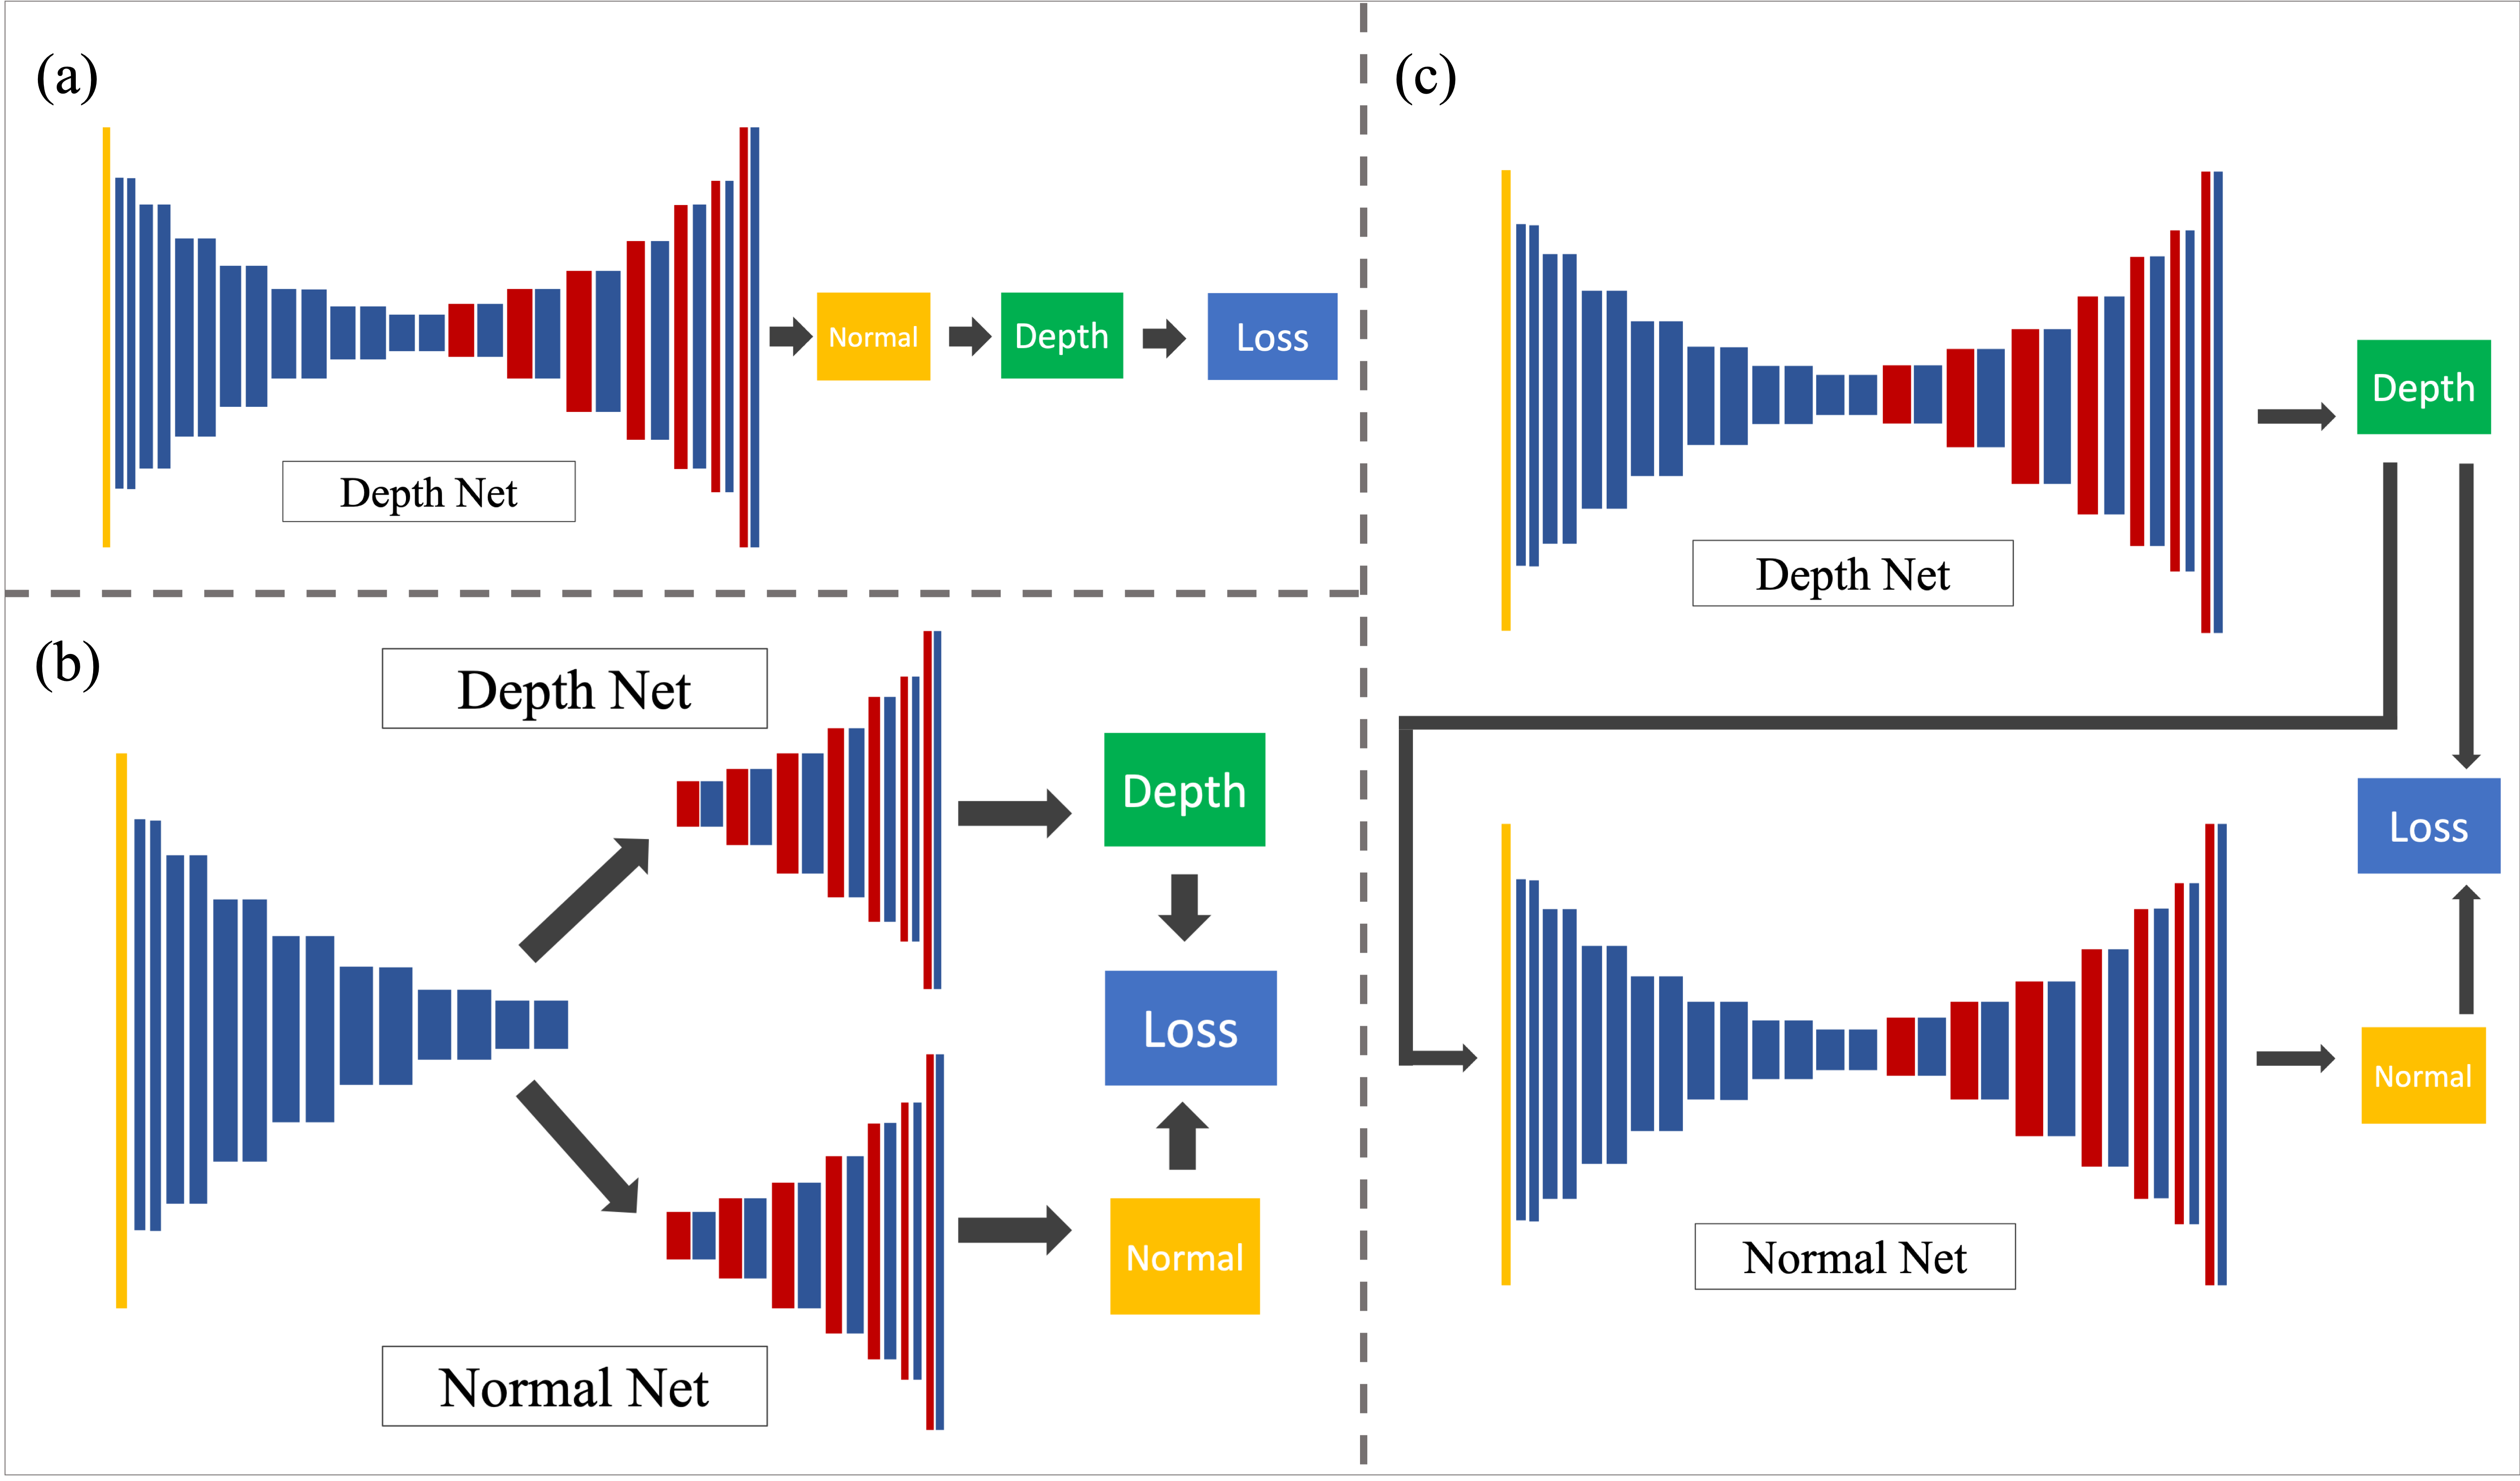
\includegraphics[width=\columnwidth ]{network.png}
  \caption{Network architectures for different experiments. (a) For the edge-aware experiments, the network architecture is based on (include related work), where we compute the normal directly from the predicted depth. (b)While evaluating the patch based photo-consistency constraints, the normal and depth net shares a single encoder and uses different decoders to separately predict depth. (c)To train the normal network with only the depth and normal orthogonality constraint, we froze the depth network and individually trained the normal network with an additional estimated depth input to get reasonable results.}
  \label{fig:network}
\end{figure}

\subsection{Datasets and metrics}
We conducted experiments on depth and normal estimation. The performances are evaluated on two popular datasets: KITTI for outdoor scene and NYUv2 for indoor scene.
For depth evaluation, we adopted those used in Zhou et al.\cite{zhou2017unsupervised}, details are shown on table\ref{table1:depth_eval}

\begin{table*}
\centering
\label{table1:depth_eval}
\begin{tabular}{l|l}
 Threshold: $\% of y_i, s.t. max(\frac{y_i}{y_i^*}, \frac{y_i^*}{y_i})=\delta < thr $&  RMSE(linear):$\sqrt{\frac{1}{|T|}\sum_{y\inT}||y_i - y_i^*||^2}$ \\
 Abs Relative difference: $\frac{1}{|T|}\sum_{y\in T||y-y^*||/y^*}$ &  RMSE(log):$\sqrt{\frac{1}{|T|}\sum_{y \in T}||log y_i - log y_i^*||^2}$ \\
 Squared Relative difference:$\frac{1}{|T|}\sum_{y\in T||y-y^*||^2/y^*}$ & 
\end{tabular}
\caption{Depth evaluation metrics}
\end{table*}

For normal evaluation, we
implement the evaluation metrics in\cite{fouhey2013data}: in addition to reporting the mean, median, and
RMSE on a per-pixel-basis, we report three pixel-accuracy
metrics, or percent-good-pixels (i.e., the fraction of pixels with cosine distance to ground-truth less than t) with $t = 11.25\degree, 22.5\degree, 30\degree$.

\subsection{Training}
Like \cite{zhou2017unsupervised}, We implemented the system using TensorFlow framework. For all the experiments, we set $\lambda_s = 0.5=l$ (l is the downscaling factor for the corresponding scale) and $\lambda_e = 0.2$. During training, we used batch normalization for all the layers except for the output layers, and the Adam optimizer with $\beta_1 = 0:9$, $\beta_2 = 0:999$, learning rate of $0.0002$ with $\%95\%$ decay and mini-batch size of 4. The training typically converges after about 150K iterations. All the experiments are performed with image sequences captured with a monocular camera. We resize the images to $128 × 416$ during training.
\\
Similar to Yang et al.\cite{yang2018lego}, we evaluate the normal map(either from direct-prediction or from depth inference) by comparing to the ground truth normal, which is generated by applying depth-to-normal layer on interpolated depth ground truth. The normal evaluation is performed
on KITTI dataset. The comparison of normal evaluations on KITTI split is presented in???. 
\subsection{Edge-aware depth experiments}
In this section we experimented edge-aware methods with the architecture shown in fig.\ref{fig:network}(a). We obtain the surface normal by directly computing from the estimated depth and calculate the loss as mentioned in \cite{yang2017unsupervised}, where it is inferred  directly from the predicted depth. For SSIM pixel loss, weight is set to 0.3. For depth edge-awareness training, we set the gradient weight to 0.5, while use the semantic mask as input to edge net and the weight is set to 0.3.
To leverage the normals in our loss function, we add an additional normal smooth loss term as we did for the depth and set the weight to 0.5. The results are shown in the \ref{table1:depth_eval}.

\subsection{Normal Net experiments}
In this section we analyze our approaches on directly predicting the surface normal qualitatively. 
\\
\textbf{Evaluation on the depth and normal orthogonalily constraint}
To evaluate the depth and normal orthogonality constraint, we first jointly train the depth and normal net by only leveraging the $L_{vs}$ and $L_{orth}$ in our loss function. Yet, the results aren't very promising (table.\ref{table1:depth_eval}). The network can not generate meaningful surface normal and also degraded the depth predictions. Thus, we independently train the normal net along with the pre-trained depth net to obtained more meaningful results(fig.\ref{fig:network}(c)). As can be seen in figure.\ref{fig:KITTI_orth}, we can roughly determine the road of the scene but geometric detail information are not observed by the network.
\\
\textbf{Evaluation on the patch-based photometric constraint}
We evaluate the patch-based photometric constraint by adding the $L_{patch}$ term in our loss function. We implement the network architecture of this experiment as shown in figure.\ref{fig:network}(b). In (fig.\ref{fig:KITTI_patch}) we show a qualitative result of this approach. As can been seen, the estimated normal could roughly capture the contours of the scene; however, there are still some spurious blob in the image. 



%------------------------------------------------------------------------
\section{Conclusion and Future Work}
Based on the notion that deep network approaches benefit from explicit geometric cues and constraints, we tried out a bunch of criteria to get better depth, normal and ego-motion prediction by offering geometric cues and set the consistency constraints. Ablation study show the results we found that take effects and those do not. \\
Future work is to try refinement methodology as explained in \cite{casser2018depth} to further improve the depth prediction. Also, improve surface normals using our best depth prediction model, 
Patch-based loss, to simultaneously improve depth and normal.
Generalize model for depth and normal prediction to other datasets like Cityscape.

\begin{figure*}
  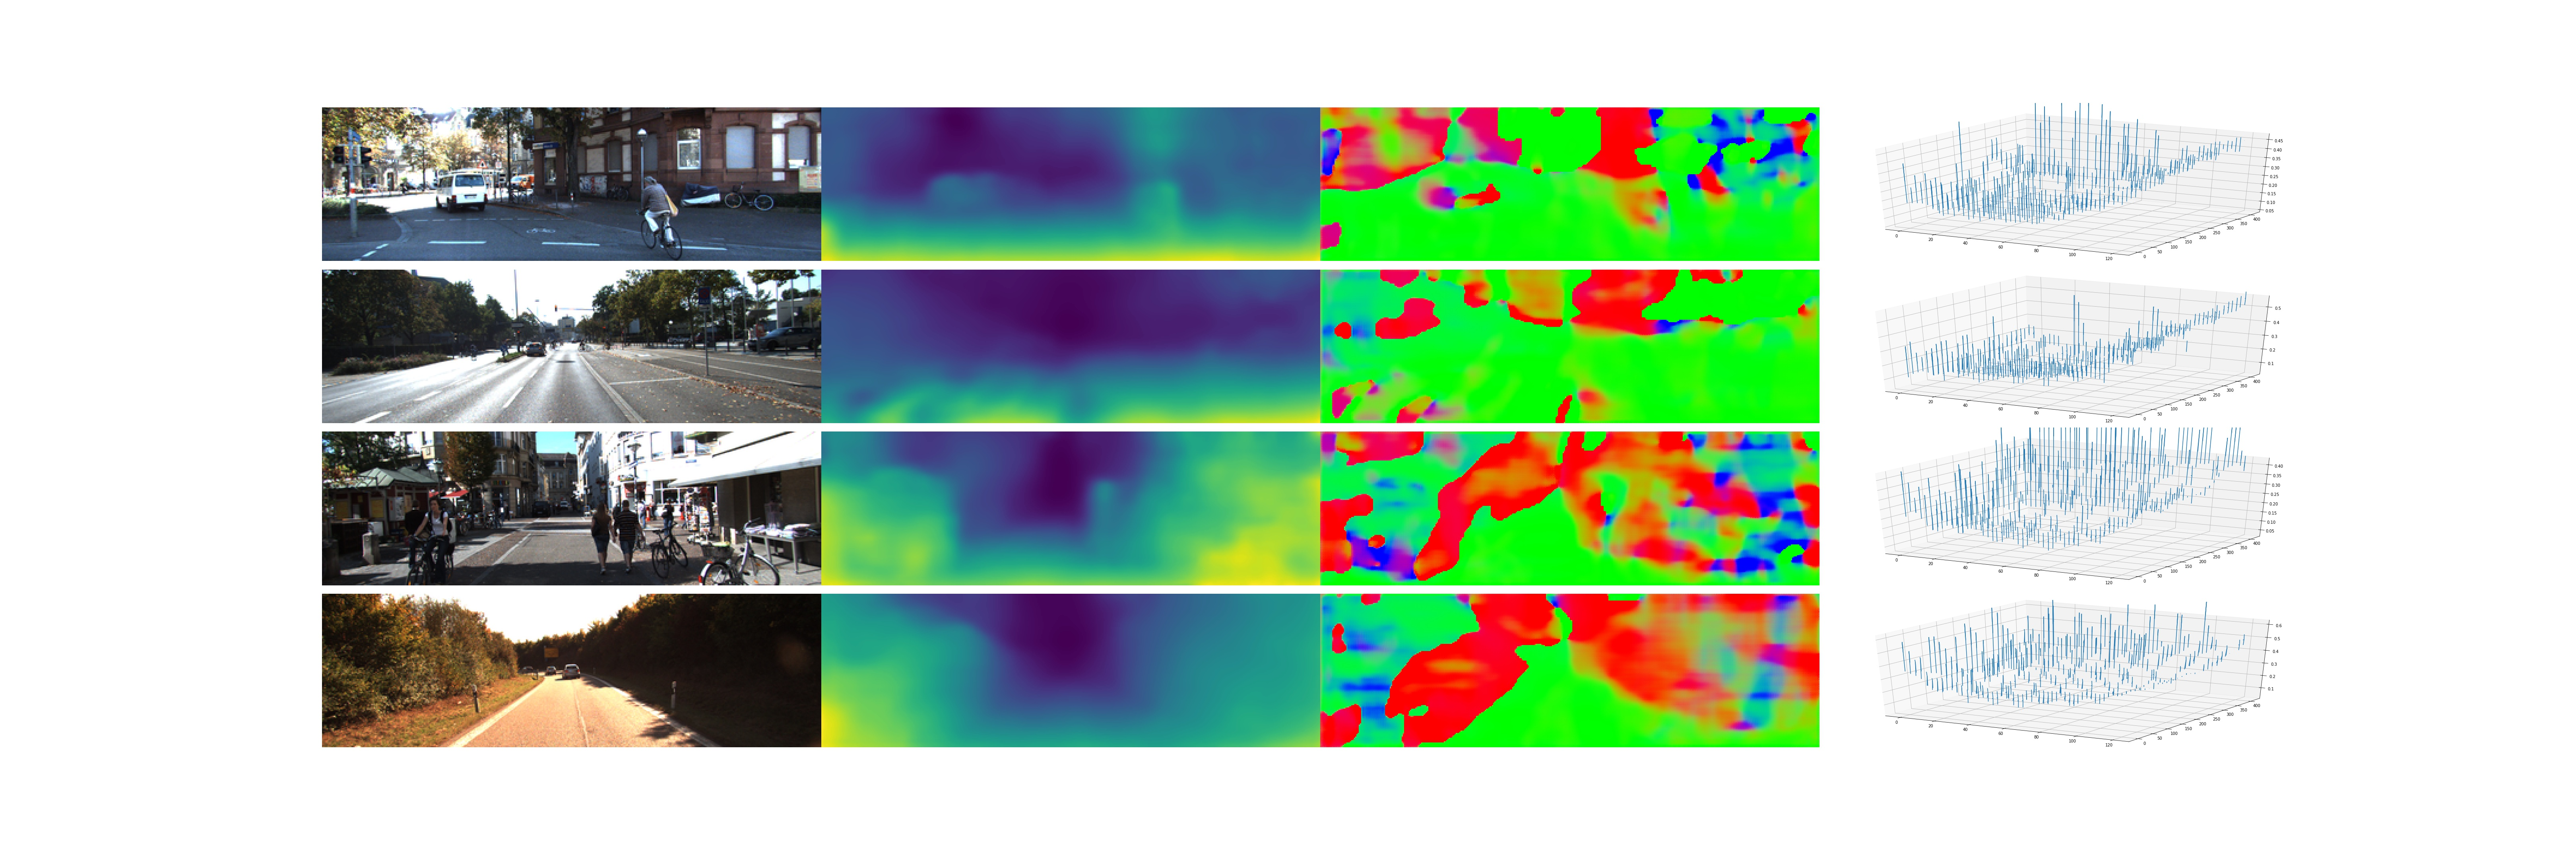
\includegraphics[width=\linewidth]{output.jpg}
  \caption{Experiment results on KITTI with only the depth and normal constraint}
  \label{fig:KITTI_orth}
  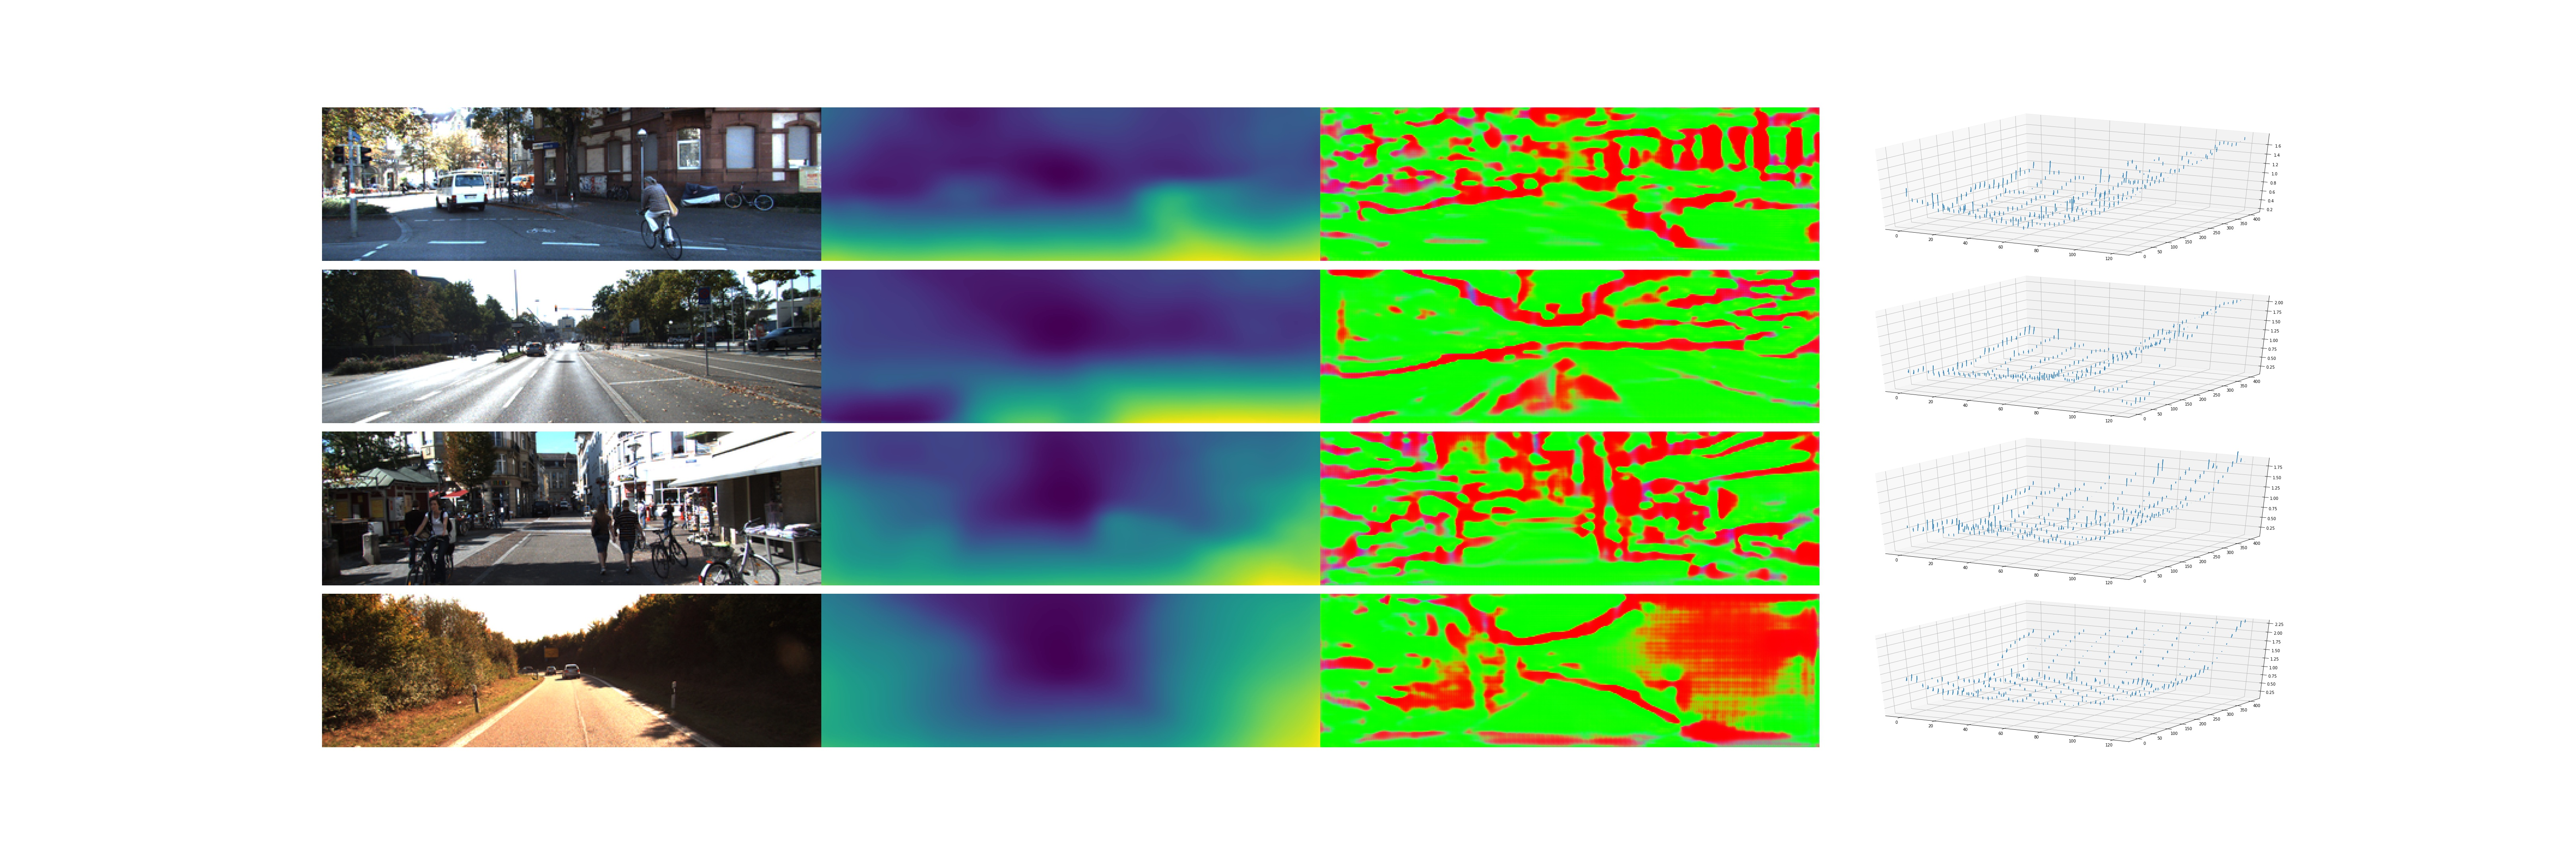
\includegraphics[width=\linewidth]{patch_based.jpg}
  \caption{Patch-based experiment results on KITTI}
  \label{fig:KITTI_patch}
\end{figure*}
%------------------------------------------------------------------------

% \begin{table}
% \begin{center}
% \begin{tabular}{|l|c|}
% \hline
% Method & Frobnability \\
% \hline\hline
% Theirs & Frumpy \\
% Yours & Frobbly \\
% Ours & Makes one's heart Frob\\
% \hline
% \end{tabular}
% \end{center}
% \caption{Results.   Ours is better.}
% \end{table}

% {\small\begin{verbatim}
%   \usepackage[dvips]{graphicx} ...
%   \includegraphics[width=0.8\linewidth]
%                   {myfile.eps}
% \end{verbatim}
% }
% \begin{figure}[t]
% \begin{center}
% \fbox{\rule{0pt}{2in} \rule{0.9\linewidth}{0pt}}
%   %\includegraphics[width=0.8\linewidth]{egfigure.eps}
% \end{center}
%   \caption{Example of caption.  It is set in Roman so that mathematics
%   (always set in Roman: $B \sin A = A \sin B$) may be included without an
%   ugly clash.}
% \label{fig:long}
% \label{fig:onecol}
% \end{figure}



% \begin{figure*}
% \begin{center}
% \fbox{\rule{0pt}{2in} \rule{.9\linewidth}{0pt}}
% \end{center}
%   \caption{Example of a short caption, which should be centered.}
% \label{fig:short}
% \end{figure*}



{\small
\bibliographystyle{ieee}
\bibliography{refs}
}

\end{document}
